% !TeX spellcheck = en_AU-EnglishAustralia
% Preamble
\documentclass[12pt, a4paper]{article}
\usepackage[utf8]{inputenc}
%\usepackage[english]{babel}

\usepackage{indentfirst}
\usepackage{rotating, graphicx}
\usepackage{geometry}
\usepackage{hyperref}
\usepackage{amsmath}
\usepackage{amssymb}
\usepackage{gensymb}
\newgeometry{vmargin={30mm}}

\title{Speaker Testing}	
\author{Laurence Prins}
\date{29.04.2021}
\usepackage[style=ieee]{biblatex}
\addbibresource{References.bib}

\begin{document}
\maketitle
\section{Class AB Amplifier (LM386)}
To start with, a circuit will be built using the class AB LM386 low voltage audio power amplifier. This was chosen as it is a readily available IC with a maximum power output equal to the maximum power input of the speaker. Being class AB it has low distortion (0.2\% at 1kHz) and low quiescent power loss (24mW with 6V supply).
\subsection{Initial Setup}
To gain an understanding of the board, the simple circuit shown in figure \ref{fig:LM386_gain_20} was constructed on a breadboard. With this circuit the gain was set to the internal value of 20. A 200$mV_{p-p}$ signal was put into $V_{in}$ and 6V was put across pin 6. 
\begin{figure} [!htb]
	\hfill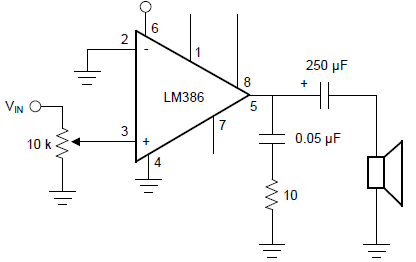
\includegraphics{./Figures/LM386_Gain_20}\hspace*{\fill}	
	\caption{LM386 audio amplifier with gain 20, source: \cite{lm386datasheet}}
	\label{fig:LM386_gain_20}
\end{figure}
\subsubsection{Results}
The result was a low sound with high distortion. Upon further inspection, the LM386 from from the store was a LM386-N1 which has a power output of 250 - 325 mW. 
\pagebreak
\subsection{Second Attempt}
The next step was to construct the circuit in figure \ref{fig:lm386Circuit} to increase the gain from 20 to 200 which can be varied using the variable resistor. The design for this amplifier is as followed:
\begin{itemize}
\item The 10k$\Omega$ variable resistor at the non inverting input acts as a volume knob, controlling the input voltage to the amplifier.
\item The 10$\mu$F and 10k$\Omega$ connected between pins 1 and 8 control the amplifier gain, with the resistor set to 0$\Omega$ then the gain is set to 20, when the resistor is set to the full 10k$\Omega$ then the gain is set to 200.
\item The 10$\mu$F ceramic capacitor connected to pin 7 is a bypass capacitor, it prevents high frequency noise from being amplified by the amplifier. 
\item At the exit of pin 5 there is a 0.68$\mu$F film capacitor and a 10$\Omega$ forming a 'Zobel network'. High frequency signals (greater than 24.5kHz) are pulled to ground preventing damage to the speaker and also providing stability to the amplifier.
\item The 220$\mu$F electrolytic capacitor before the speaker acts to remove the DC bias from the signal into the speaker. The capacitor forms a high pass filter with the 8$\Omega$ speaker, electrolytic capacitors are capable of having much higher capacitances than other capacitors, thus the capacitor here is chosen as electrolyic to allow the lower frequencies through. 
\end{itemize}
\begin{figure}[!htb]
	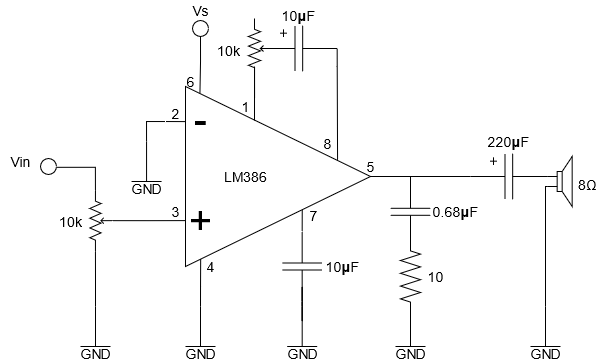
\includegraphics[width=0.5\textwidth]{./Figures/Class_AB_Amp}
	\includegraphics[width=0.5\textwidth]{./Figures/Class_AB_Amp_Physical}	
	\caption{Circuit diagram for the class AB amplifier circuit using the LM386 (left) and the physical implementation (right)}
	\label{fig:lm386Circuit}
\end{figure}
\pagebreak
\section{Class D Amplifier (PAM8403)}
The current system utilises the class D amplifier PAM8403 which came in a pre-built PCB intended for use with interfacing with the Arduino. This makes it ideal for our use as we can get the high power and efficiency of the class D amplifier without having to go out of our way to manufacture our own PCB thus saving time. This PCB is shown in figure \ref{fig:classDAmp}. 
\begin{figure} [!htb]
	\hfill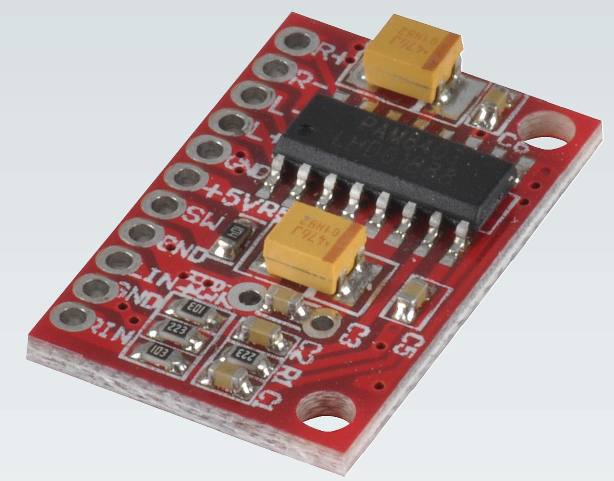
\includegraphics[width=0.5\textwidth]{./Figures/Class_D_Amp_Physical}\hspace{\fill}
	\caption{Class D audio amplifier PCB}
	\label{fig:classDAmp}
\end{figure} \\
The downside of using this PCB is that it does not include an output low pass filter. As previously explained, class D amplifiers are switching amplifiers, and as such output waveform will be square. This is relevant for when using sine waves in a following section for producing sinusoidal waveforms. \\

This amplifier has differential outputs of type BD and thus the block diagram can be drawn with these differential outputs.

\pagebreak
\section{Programming}
The chosen microcontroller is the Teensy 4.0. This has the benefit of a fast clock speed (up to 600Mhz) and is easily programmed using the Arduino IDE. Each pin has an output of 3.3V with a 4mA maximum current. \\
\subsection{Initial Programming}
The Arduino libraries come with an inbuilt 'tone' function which plays a 50\%
duty cycle PWM waveform with a chosen frequency. The first test code waited to receive a 'P' through serial and played a waveform of the chosen frequency.
\subsection{Further Development}
Further development allowed the user to specify the frequency, wave time and the number of pulses directly into serial. It did this by taking in a three column array with the field [freq,toneLength, number of pulses] and produces a tone with those properties. 
\subsection{Even Further Development}
The current code is completely encapsulated within the serial interface. Users can create "Waveforms" with the following properties:
\begin{itemize}
	\item Initial Frequency
	\item Final Frequency
	\item Waveform Time: The amount of time to play the waveform in milliseconds
	\item Waveform Pulses: The number of times the waveform will be played for.
	\item Waveshape: The shape of the wave, options are: square (p) or sine (s).
\end{itemize}
Each waveform is given a unique identifier and is stored in a singly linked list data structure which can be visualised as in figure \ref{fig:linkedLists}.
\begin{figure} [!htb]
	\hfill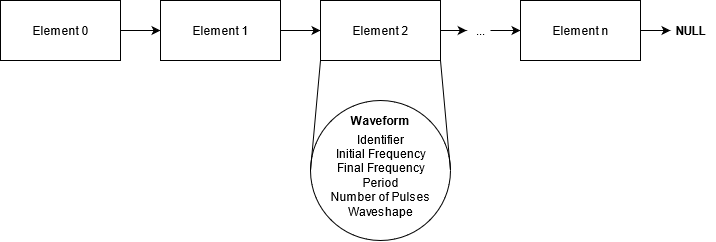
\includegraphics[width=0.8\textwidth]{./Figures/Linked_Lists}\hspace{\fill}
	\caption{Visualising linked list data structure with the "waveforms"}
	\label{fig:linkedLists}
\end{figure} 
\pagebreak

\subsection{Serial Commands}
If given an invalid command, the code will spit out an error which will prevent the microcontroller from locking up.
\subsubsection{New Waveform}
To create a new waveform type the following:
\begin{center}
	$<$n(f,t,n,s)$>$
\end{center} 
Where f = frequency in Hz, t = time in ms, n = \# pulses, and s = wave shape.\\
Spits out an error if not given a valid 4 inputs. Creates a waveform with the specified properties and inserts it at the next free link in the linked list.
\subsubsection{Edit Waveform}
To edit an already created waveform in the linked list type the following: \\
\begin{center}
	$<$e(i,p,new\_value)$>$
\end{center}
Where i = waveform identifier, p = property (f0, f1, time, pulses, shape), new\_value = new value for the specified property. \\

Can edit multiple properties at once.
\subsubsection{Delete Waveform}
To remove a waveform type the following: \\
\begin{center}
	$<$r(i)$>$
\end{center}
Where i = identifier. Can input i = a to remove all the waveforms. \\
Removes the waveform from the linked list and reserves its slot. 
\subsubsection{Display Waveform}
\begin{center}
	$<$d(i)$>$
\end{center}
Where i = identifier. Can input i = a to display all the waveforms in the list. \\
Displays the waveform in the serial monitor. 
\subsubsection{Play Waveform}
\begin{center}
	$<$p(i)$>$
\end{center}
Where i = identifier. \\
Plays the specified waveform through the AUDIO\_OUTPUT pin. 
\subsubsection{Loop Waveform}
\begin{center}
	$<$l(i)$>$
\end{center}
Where i = identifier. \\
Plays the specified waveform through the AUDIO\_OUTPUT pin. Can stop the loop by inputting a new command into serial. 

\subsection{Transmitter Commands}
To get the speaker ready to transmit, new commands were added. 
\subsubsection{Configure Transmitter}
\begin{center}
	$<$TxCfg(p1,v1,p2,v2,...,pn,vn)$>$
\end{center}
Configure the transmitter with the specified values. i = identifier of waveform. pn = property (pin, waveform, or delay). vn = new value.

\subsubsection{Display Transmitter}
\begin{center}
	$<$TxDisp()$>$
\end{center}
Prints all the current properties of the transmitter into the serial monitor.

\subsubsection{Transmit}
\begin{center}
	$<$Tx()$>$
\end{center}

\begin{enumerate}
	\item Pulls the transmitter pin high
	\item Transmits the specified waveform through the AUDIO\_OUTPUT pin.
	\item Waits delay period.
	\item Pulls pin low.
\end{enumerate}

\subsection{Play Tone Commands}
\subsubsection{Play Tone}
\begin{center}
	$<$pt(f0,f1,t,s)$>$
\end{center}
Plays a tone with the specified properties through the audio output pin. if f0 $\neq$ f1 then this will play a linear FM sweep between those frequencies. f0 = initial frequency [Hz].
f1 = final frequency [Hz]. t = wave time [s]. s = waveshape (s = sinusoidal, p = square).
\subsubsection{Loop Tone}
\begin{center}
	$<$pt(f0,f1,t,s)$>$
\end{center}
Plays a tone with the specified properties through the audio output pin until the serial reads a new input. f0 = initial frequency [Hz]. f1 = final frequency [Hz]. t = wave time [s]. s = waveshape (s = sinusoidal, p = square).

\pagebreak
\section{Generating a Sine Wave}
The Teensy 4.0 does not come with an on board DAC. To generate a sinusoid to feed to the speaker can either use an off board DAC or can generate a sine wave estimate through code using PWM.
\subsection{Sinusoidal PWM}
Can estimate a sine wave by varying the duty cycle of a PWM waveform and passing this waveform through a low pass filter. The system can be drawn as such in figure \ref{fig:SystemPreLPF}.
\begin{figure} [!htb]
	\hfill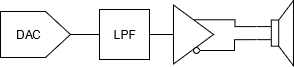
\includegraphics[width=0.5\textwidth]{./Figures/System_Pre_LPF}\hspace{\fill}
	\caption{Block diagram for the system with a DAC and class D amplifier}
	\label{fig:SystemPreLPF}
\end{figure}

\subsubsection{Method}
We are estimating a sine wave period $T_s$ by dividing it up into $L$ discrete intervals. At each of these intervals, vary the duty cycle of the PWM waveform. The PWM duty cycles can be put into a sine look up table (LUT) of length L with the maximum value equal to $2^m - 1$ where m is the resolution of the PWM waveform which corresponds to 100\% duty cycle. The minimum value in the look up table is 0 which corresponds to 0\% duty and the mid point $(2^m-1)/2$ is 50\% duty. 

\begin{figure} [!htb]
	\hfill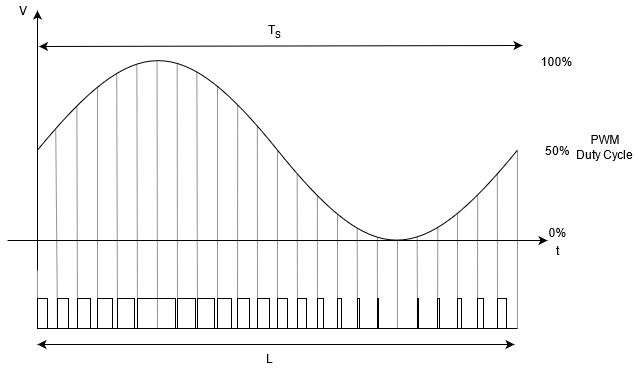
\includegraphics[width=0.9\textwidth]{./Figures/Sinusoidal_PWM}\hspace{\fill}
	\caption{Sinusoidal PWM generation through code}
	\label{fig:sinusoidalPWM}
\end{figure}

To determine the rate which we go through the LUT, use a counter and an interrupt timer. At each interrupt period, $\tau$, add a step value of $\Delta$ to the current counter value and once the counter exceeds the maximum value, $M$, reset the counter and carry the remainder. This is demonstrated in figure \ref{fig:sinusoidalPWMCounter}. 
\begin{figure} [!htb]
	\hfill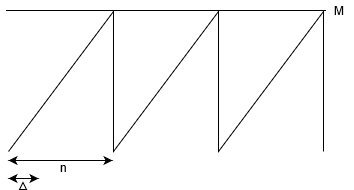
\includegraphics[width=0.7\textwidth]{./Figures/Counter}\hspace{\fill}
	\caption{Counter}
	\label{fig:sinusoidalPWMCounter}
\end{figure}

It takes $n$ intervals to exceed $M$ therefore:
\begin{equation}
	n\times\Delta \ge M \implies n = \frac{M}{\Delta}
	\label{eqn:M/D}
\end{equation}

Calling an interrupt every $\tau$ seconds and so the time it takes per increment of the LUT is $n\times T$. And there are $L$ elements in the table so, per sine period it takes:
\begin{equation}
	T_s = n\times \tau\times L
\end{equation}
Which can be written in terms of frequency:
\begin{equation}
	f_s = \frac{1}{\tau nL}
\end{equation}
And in terms of the step size by substituting equation \ref{eqn:M/D}:
\begin{equation}
	f_s = \frac{\Delta}{M\tau L}
\end{equation}
The values that are currently used are:
\begin{itemize}
	\item M = 100
	\item $\tau$ = 5$\mu$s
	\item L = $2^8$
	\item m = 8
\end{itemize}
This is the frequency of the sinusoidal waveform. The PWM waveform needs a much higher frequency than the sine frequency. The system currently use a PWM frequency of $f_{PWM} = f_s \times L$ though this can be reduced to $f_{PWM} = f_s \times 40$ if necessary based on hardware constraints.\\

This waveform then needs to fed into a low pass filter to smooth the waveform and form a sine wave. Current system uses a first order RC low pass filter with a cut-off frequency of 19.9kHz. The RC low pass filter is shown in figure \ref{fig:RCLPF1}.
\begin{figure} [!htb]
	\hfill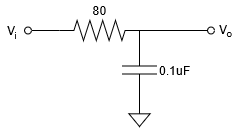
\includegraphics[width=0.5\textwidth]{./Figures/RC_LPF}\hspace{\fill}
	\caption{First order RC low pass filter design with $f_c = 19.9kHz$}
	\label{fig:RCLPF1}
\end{figure}

\subsubsection{Results}
Probing the output of the LPF and varying the frequency yields the graphs shown in figures \ref{fig:sine1kHz2kHz}, \ref{fig:sine3kHz4kHz} and \ref{fig:sine5kHz}. This method works for frequencies up to 5kHz before the equations start to fall apart. 

\begin{figure} [!htb]
	\hfill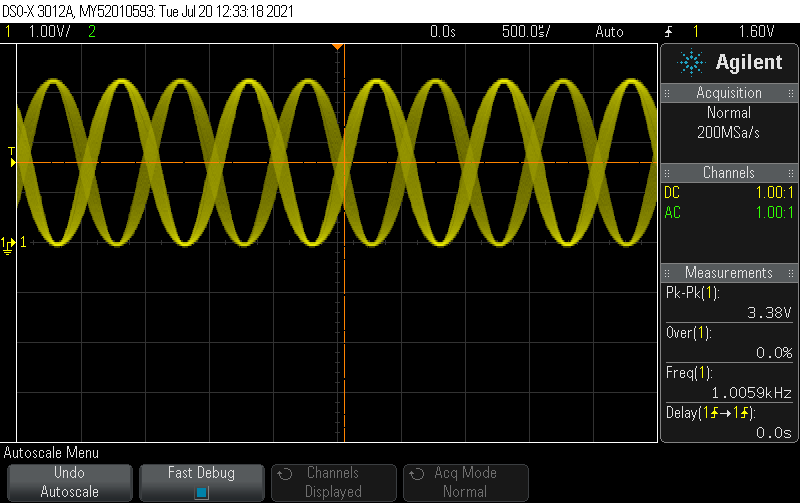
\includegraphics[width=0.35\textwidth]{./Figures/Sine_1kHz}\hspace{\fill}
	\hfill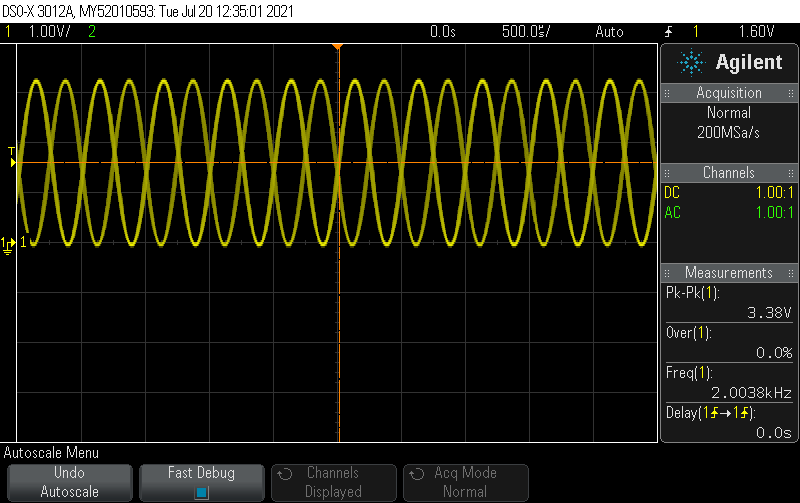
\includegraphics[width=0.35\textwidth]{./Figures/Sine_2kHz}\hspace{\fill}
	\caption{1kHz (left) and 2kHz (right) sinusoids}
	\label{fig:sine1kHz2kHz}
\end{figure}

\begin{figure} [!htb]
	\hfill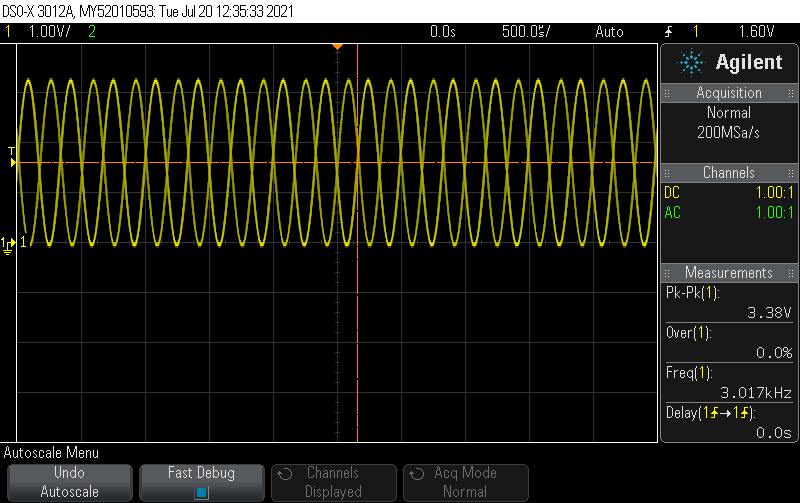
\includegraphics[width=0.35\textwidth]{./Figures/Sine_3kHz}\hspace{\fill}
	\hfill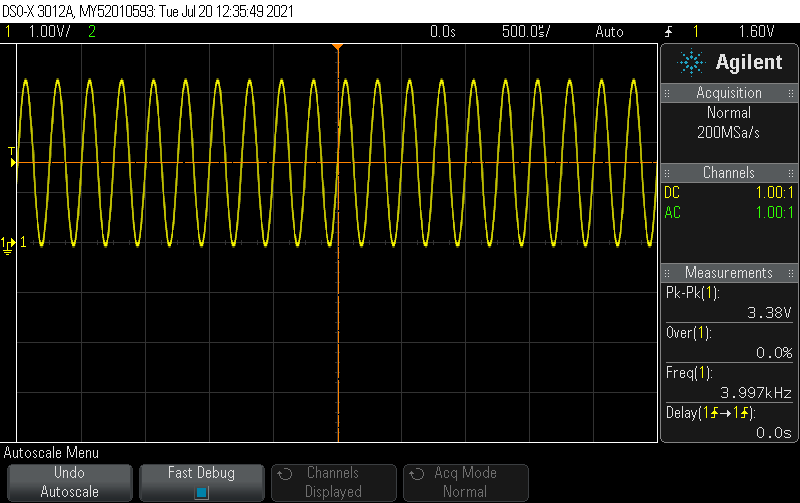
\includegraphics[width=0.35\textwidth]{./Figures/Sine_4kHz}\hspace{\fill}
	\caption{3kHz (left) and 4kHz (right) sinusoids}
	\label{fig:sine3kHz4kHz}
\end{figure}

\begin{figure} [!htb]
	\hfill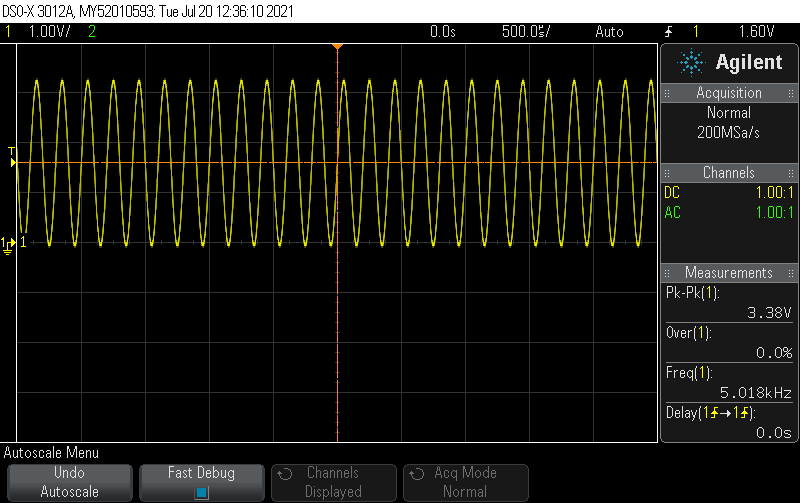
\includegraphics[width=0.35\textwidth]{./Figures/Sine_5kHz}\hspace{\fill}
	\caption{5kHz sinusoid}
	\label{fig:sine5kHz}
\end{figure}
\pagebreak
\section{Linear FM Sweep (chirp)}
The equation for a linear FM chirp is:
\begin{equation}
	f(t) = ct + f_0
\end{equation}
Where $f_0$ is the initial frequency, c is the chirp rate calculated as:
\begin{equation}
	c = \frac{f_1 - f_0}{T}
\end{equation}
Where $f_1$ is the final frequency, T is the sweep time. \\
\subsection{Square Chirp}
Can call an interrupt every $\tau$ seconds which will increase the current frequency. If the waveform plays for T seconds then the number of interrupts that are called within that time frame is:
\begin{equation}
	n = \frac{T}{\tau}
\end{equation}
Can use this to determine the frequency step that will be added onto the current frequency at the next interrupt call.
\begin{equation}
	\Delta f = \frac{f_1 - f_0}{n}
\end{equation}
\subsection{Sinusoidal Chirp}
Same method as before except using the frequency steps, at each interrupt the frequency step is added to the current frequency step. The "frequency step step" is then:
\begin{equation}
	\Delta_\Delta = \frac{\Delta_1 - \Delta_0}{n} 
\end{equation}
Where:
\begin{equation*}
	\Delta_1 = f_1ML\tau
\end{equation*}

\begin{equation*}
	\Delta_0 = f_0ML\tau
\end{equation*}

\begin{equation*}
	n = \frac{T}{\tau}
\end{equation*}
\pagebreak

\section{Class D Amplifier Cont.}
Recall that the class D amplifier is a switching amplifier. This means that the outputted waveform is a square waveform, so the work done in the previous section is undone by the amplifier. Therefore, need to include another low pass filter at the exit of the amplifier. The system block diagram can be redrawn as such in figure \ref{fig:SystemPostLPF}.
\begin{figure} [!htb]
	\hfill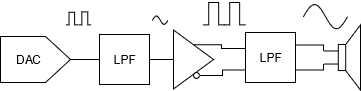
\includegraphics[width=0.5\textwidth]{./Figures/System_Post_LPF}\hspace{\fill}
	\caption{Block diagram for the system with a DAC and class D amplifier and a LPF at the exit of the amplifier}
	\label{fig:SystemPostLPF}
\end{figure} \\
For the 8 $\Omega$ speaker, it is recommended to implement a second order Butterworth LC filter shown in figure \ref{fig:Speaker_LPF}. 

\begin{figure} [!htb]
	\hfill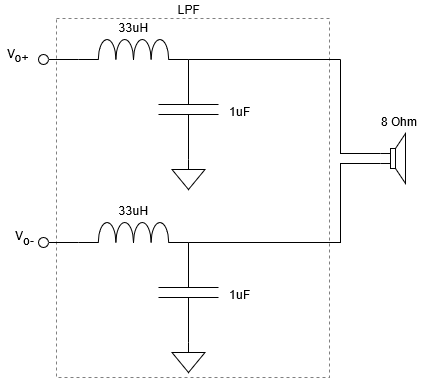
\includegraphics[width=0.5\textwidth]{./Figures/Speaker_LPF}\hspace{\fill}
	\caption{2nd order Butterworth LC filter as recommended by Texas instruments}
	\label{fig:Speaker_LPF}
\end{figure}
\pagebreak
\subsection{Results}
After implementing the LC filter as shown in figure \ref{fig:Speaker_LPF}, the outputted waveform was still square as shown in figure \ref{fig:stillSquare}. 
\begin{figure} [!htb]
	\hfill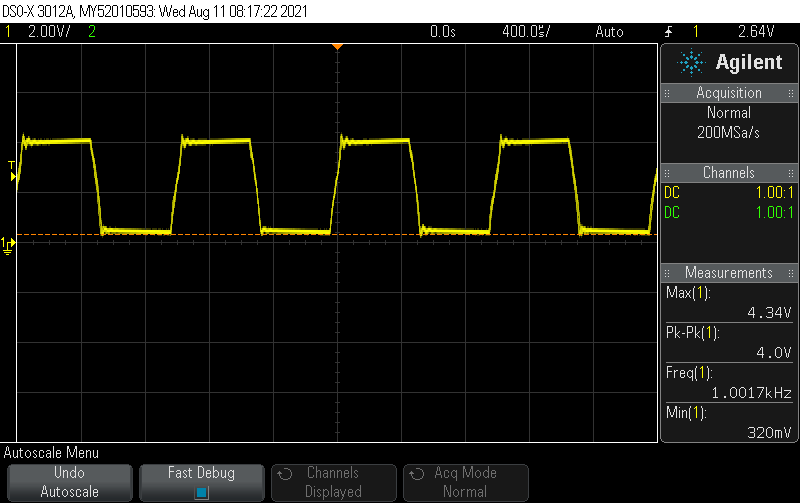
\includegraphics[width=0.5\textwidth]{./Figures/Waveforms/Output_Class_D_Filtered}\hspace{\fill}
	\label{fig:stillSquare}
	\caption{Output waveform as produced with an inputted 3.3V pk-pk sinusoidal waveform}
\end{figure}
It is clear that something was wrong. It took an embarrassingly long time to work out that the problem was not necessarily the low pass filter, it was the waveform being clipped on the input of the amplifier. \\

The amplifier has a maximum input voltage rating of -0.3V to 0.3V, It was being fed -1.65 to 1.65V and so the tops of the waveforms were being cut off. This can easily be fixed by implementing a variable resistor to create a voltage divider at the input of the amplifier. Same as what was done with the LM386 amplifier. This is implemented in figure \ref{fig:SpeakerAndAmplifier} where the voltage divider is a 10k variable resistor to act as a volume knob. \\

With the voltage divider made the output waveforms now look more like a sinusoid see figure \ref{fig:nowSinusoid}. There is just the issue of the zero-crossing distortion. The waveform is also not centred around ground and so there is less output power so the speaker sounds quiet. To fix this, a DC blocking capacitor can be added to shift the waveform back to DC.


\begin{figure}[!htb]
	\hfill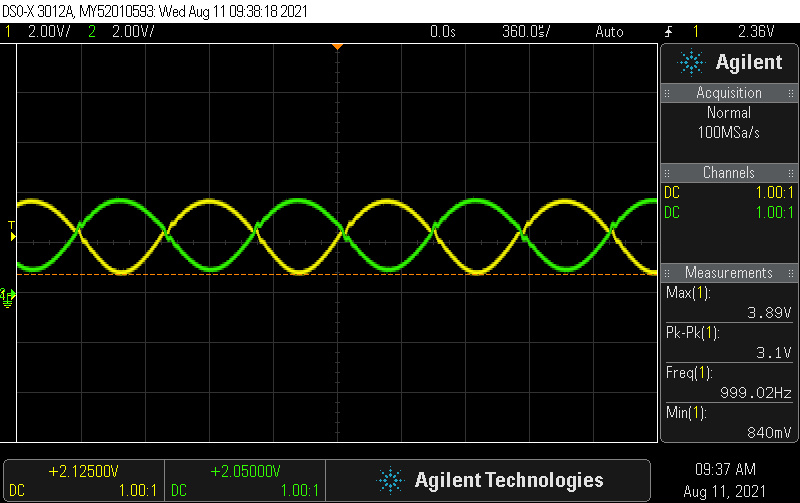
\includegraphics[width=0.5\textwidth]{./Figures/Waveforms/Output_Class_D_Filtered_Reduced_Input (2)}\hspace{\fill}
	\label{fig:nowSinusoid}
	\caption{Output waveform as produced with an inputted 0.6V pk-pk sinusoidal waveform, yellow is connected to speaker positive terminal and green is connected to speaker negative terminal}
\end{figure}

\begin{figure}[!htb]
	\hfill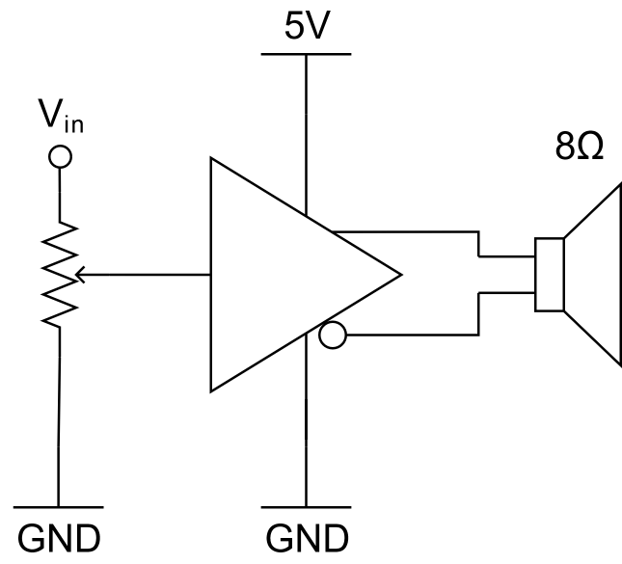
\includegraphics[width=0.5\textwidth]{./Figures/Amplifier_And_Speaker}\hspace{\fill}
	\label{fig:SpeakerAndAmplifier}
	\caption{Class D amplifier and speaker with a variable resistor at entrance to the amplifier to act as a volume knob.}
\end{figure}

\section{Final Speaker Hardware Design and Results}
The final schematic for the system is shown in figure \ref{fig:FinalSchematic} This implements all of the hardware fixes identified from the previous section. This system is capable of playing sinusoids of up to 20kHz, the full range of the speaker. It turns out that the speaker does not need the output Butterworth LC filter outlined in section 6 as the speaker itself acts as a low pass filter. 
\begin{figure}[!htb]
	\hfill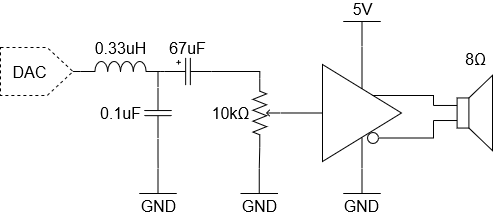
\includegraphics[width=\textwidth]{./Figures/System_Full_Schematic}\hspace{\fill}
	\label{fig:FinalSchematic}
	\caption{Full schematic of the system}
\end{figure}

Figure \ref{fig:VerySmooth} shows the waveform as produced at the exit of the LPF before the DC blocking capacitor. This is much smoother than what was shown in figure \ref{fig:sine1kHz2kHz}.
\begin{figure}[!htb]
	\hfill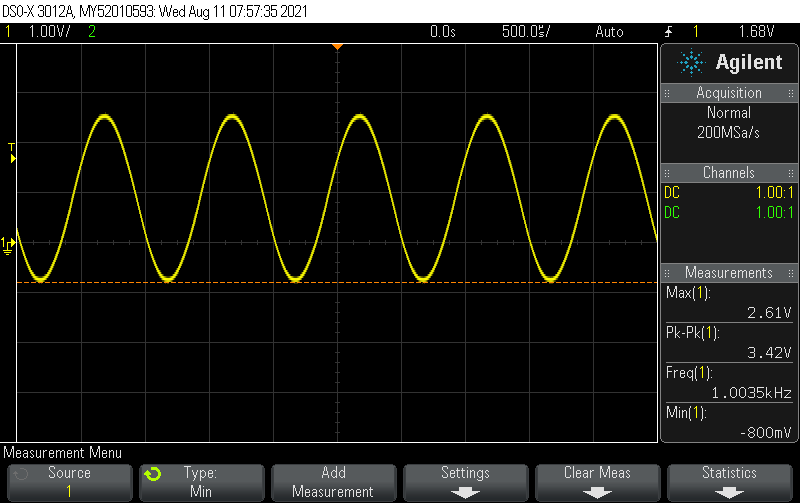
\includegraphics[width=\textwidth]{./Figures/Waveforms/LC_Filtered_Sinewave (2)}\hspace{\fill}
	\label{fig:VerySmooth}
	\caption{Playing a 1kHz tone as extracted from the exit of the LPF}
\end{figure}

\section{Testing Waveforms}
\subsection{Analogue Microphone (AM4011)}
An analogue microphone can be set up to test the waveform purity of the speaker and amplifier system. To do this a circuit very similar to the speaker amplifier circuit in section 1.2 is built where the output of the microphone is connected to the input of the amplifier. The circuit diagram is shown in figure \ref{fig:microphoneAmplifier} and has the following design considerations:
\begin{itemize}
	\item The microphone requires power to operate, R1 acts to supply this power. The chosen microphone is the AM4011 which has an operation voltage of 1.5 to 15 V dc and a current consumption of 0.8mA at 6V supply. Using ohm's law, to supply 0.8mA to the microphone the chosen value of R1 is 6.5k$\Omega$. (currently using 10k).
	\item C1 acts to remove the DC from the microphone since we just want the AC output from the microphone going into the amplifier input.
	\item The 10k$\Omega$ variable resistor R2 at the non inverting input acts as a volume knob, controlling the input voltage to the amplifier.
	\item The 10$\mu$F capacitor C2 and the 10k$\Omega$ resistor R3 connected between pins 1 and 8 control the amplifier gain, with the resistor set to 0$\Omega$ then the gain is set to 20, when the resistor is set to the full 10k$\Omega$ then the gain is set to 200.
	\item The 10$\mu$F ceramic capacitor C3 connected to pin 7 is a bypass capacitor, it prevents high frequency noise from being amplified by the amplifier. 
	\item At the exit of pin 5 there is a 0.68$\mu$F film capacitor C4 and a 10$\Omega$ resistor R4 forming a 'Zobel network'. High frequency signals (greater than 24.5kHz) are pulled to ground preventing damage to the speaker and also providing stability to the amplifier.
	\item The 220$\mu$F electrolytic capacitor C5 before the speaker acts to remove the DC bias from the signal into the speaker. 
\end{itemize}
\begin{figure}[!htb]
	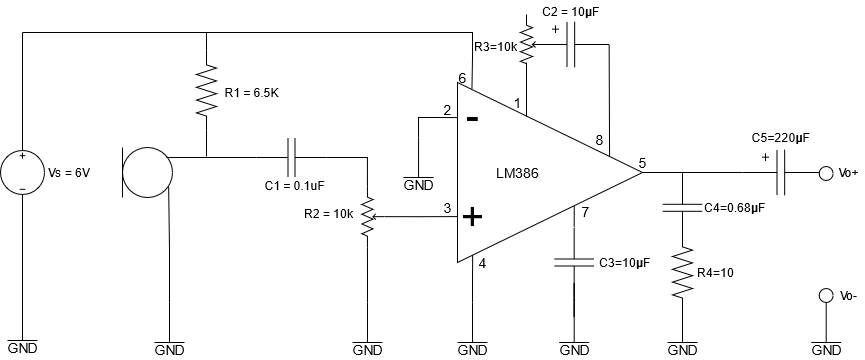
\includegraphics[width=\textwidth]{./Figures/Analogue_Microphone_Circuit}	
	\caption{Microphone amplifier circuit}
	\label{fig:microphoneAmplifier}
\end{figure}
\subsection{To Do}
\begin{itemize}
	\item Debug the microphone circuit, currently does not work.
\end{itemize}
\printbibliography[title={References}]
\end{document}